\chapter{Memory Hierarchy}

\section{L3 Cache Slicing}

\todoms{Add a plot to check if and how L3 Cache slices are distributed around the CPU. Cite McCaplin.}
\todoms{What is the Hashing algorithm?
Are all CHA boxes used for L3 Cache slices?
Increase the size of the allocated memory. Use hugetables.
Is this a CPU architecture problem or a linux problem?}

\begin{figure}[]
    \centering
    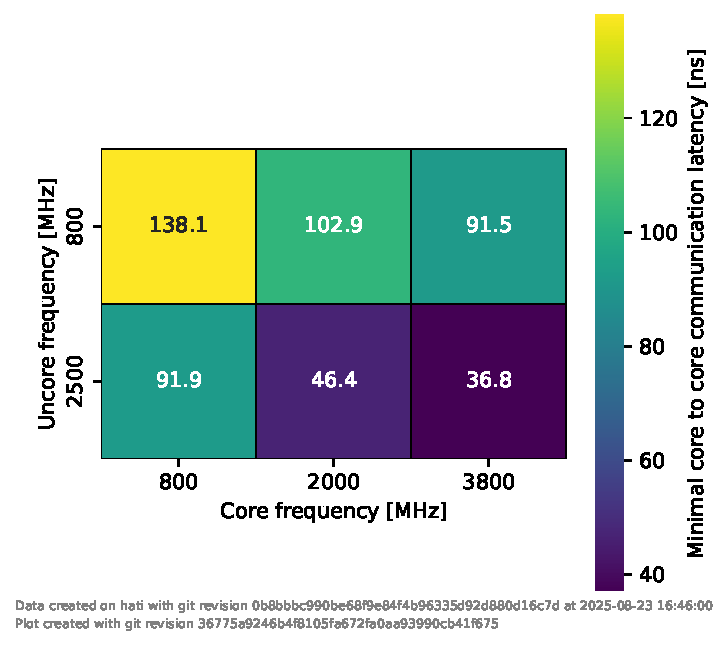
\includegraphics[width=\columnwidth]{fig/core-to-core-latency/all-to-all-heatmap-min.pdf}
    \caption{Minimal core to core communication latency over all cores of hati's socket 0.}
\end{figure}
\begin{figure}[]
    \centering
    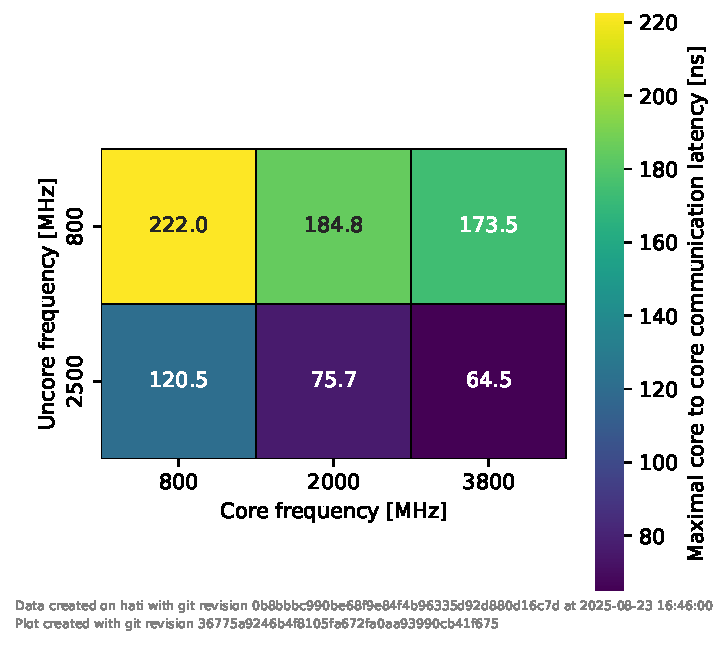
\includegraphics[width=\columnwidth]{fig/core-to-core-latency/all-to-all-heatmap-max.pdf}
    \caption{Maximal core to core communication latency over all cores of hati's socket 0.}
\end{figure}
\begin{figure}[]
    \centering
    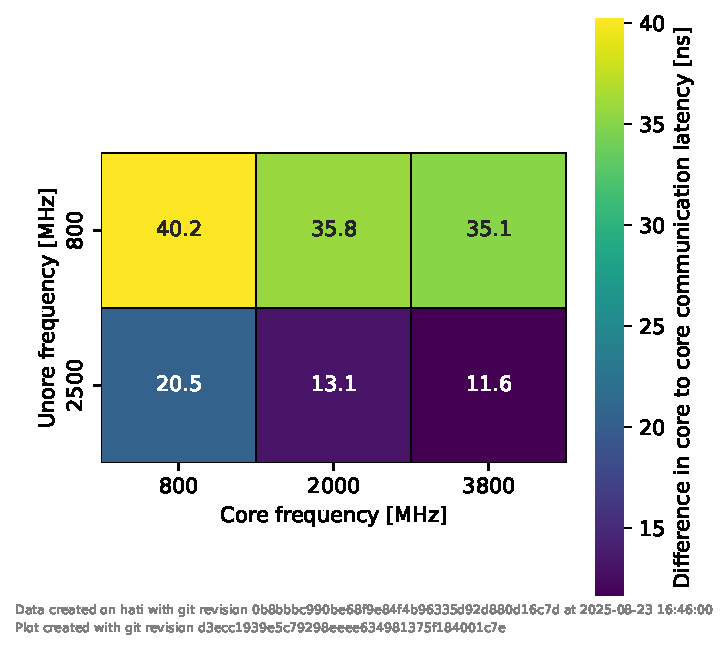
\includegraphics[width=\columnwidth]{fig/core-to-core-latency/all-to-all-heatmap-diff.pdf}
    \caption{Difference in core to core communication latency over all cores of hati's socket 0.}
\end{figure}


\section{Cache Latencies and Bandwidth}

\todoms{Reference Laukemann et al. D. Write-Allocate Evasion}